
\documentclass[conference]{IEEEtran}
\usepackage[utf8]{inputenc}
\usepackage[english]{babel}
\usepackage{graphicx}
\usepackage{amsmath}
\usepackage{hyperref}
\usepackage{natbib}
\usepackage{geometry}
\geometry{margin=1in}

\title{Deterministic Random Bit Generators based on bee position identification with deep learning x}
\author{Tomas Bedoya \\
Daniel Andre Jaime Cárdenas  \\
Eder Leandro Carbonero Baqueron \\}
\date{\today}

\begin{document}

\maketitle
\begin{abstract}
Aquí va el resumen del artículo, una breve descripción del problema, la metodología y los resultados.
\end{abstract}

\section{Introduction}
Due to the deterministic nature of traditional computers, which is what most people and appliances use to this day and will continue being so for the foreseeable future, Random Number Generation (RNG) has proven to be a challenge. Due to the reliance of cryptographic algorithms, communication protocols and other security systems in random values, there’s a constant race to find ever-better sources of randomness that follow the international standards of quality; the higher the randomness of a source, the greater the security it provides. This proves to be a challenge, however, for true randomness is difficult to find. Computers themselves cannot produce it and rely on Pseudo Random Number Generation (PRNG) to simulate random values. Other techniques, such as finding random measurements on certain like the time between user key strokes or mouse movements have proven to be unsatisfactory when put under statistical scrutiny (Mechalas, 2018). 
To guarantee that sensible processes utilize proper random sources, the NIST structured the SP 800-90 Standards for Random Number Generation (RNG) for safe RNG in cryptographic contexts. The following sections delve deep into several RNG methods, both of pseudo and true randomness, that follow these standards. They explore the different entropy sources they use (or don’t), analyses how they extract random number chains from them, and evaluate the quality of their randomness through a series of statistical evaluations. Our aim is to understand better where RNG stands today, to evaluate how they fare against each other, and determine which of these methods work better for which applications.


\section{methodologies}
\section{Methology}
\subsection{Random Number Generation}
\label{sec:random_generation}

For this exercise, three different forms of random number generation were performed. The first was through the \textit{CTR\_DRBG} algorithm, which used random keys generated by the \texttt{random} function of the Python programming language version 3.9 as seeds and was executed on a MacBook Pro M3 Pro computer. This detail may lead to different results if the experiment is replicated. However, we assume that Python's \texttt{random} function generates a uniform randomness distribution, simulating an entropic system for generating random bits.

For the second option, a sequential range of seeds was chosen, which were formatted in 32 bits to ensure compatibility with AES encryption. The sequence started at 1 and increased by one until reaching 50 million seeds. These seeds were then used to execute the \textit{CTR\_DRBG} algorithm, which generates the pseudo-random bit values.

The third approach made use of the Beacon system. In this case, the official NIST API was consumed to retrieve the last 15,600 random bits, generated from 512-bit values, obtained from the historical records maintained by the system.


\section{Results}
\subsection{Histogram analysis}
\label{sec:histogram_analysis}

\subsection{Distribution of Random Bits Generated with Python Random Seeds}
\label{sec:distribution_python_seed}

The distribution results of each technique are separated by the method used to obtain the seed versus the technique used to distill and obtain the random big number, so we can observe different results for each case.

To view the distribution of values, distribution graphs were used, either standard or uniform, depending on the input data. In our experiments, uniform distributions were shown. 8-bit segments were taken, dividing the entire input data set into byte blocks, obtaining bytes from 0 to 255. This range of possibilities gives us a visual of how the results are distributed.

We begin with the first technique, which was the generation of 6.25 million 32-byte seeds that were used to generate 6.25 million random bytes, or 50 million random bits, using the \textit{CTR\_DRBG} technique. The graph we see below leads us to the conclusion that there is a uniform distribution of the results without pronounced peaks, which are a symptom of an effective system in generating random bits.

\begin{figure}[htbp]
    \centering
    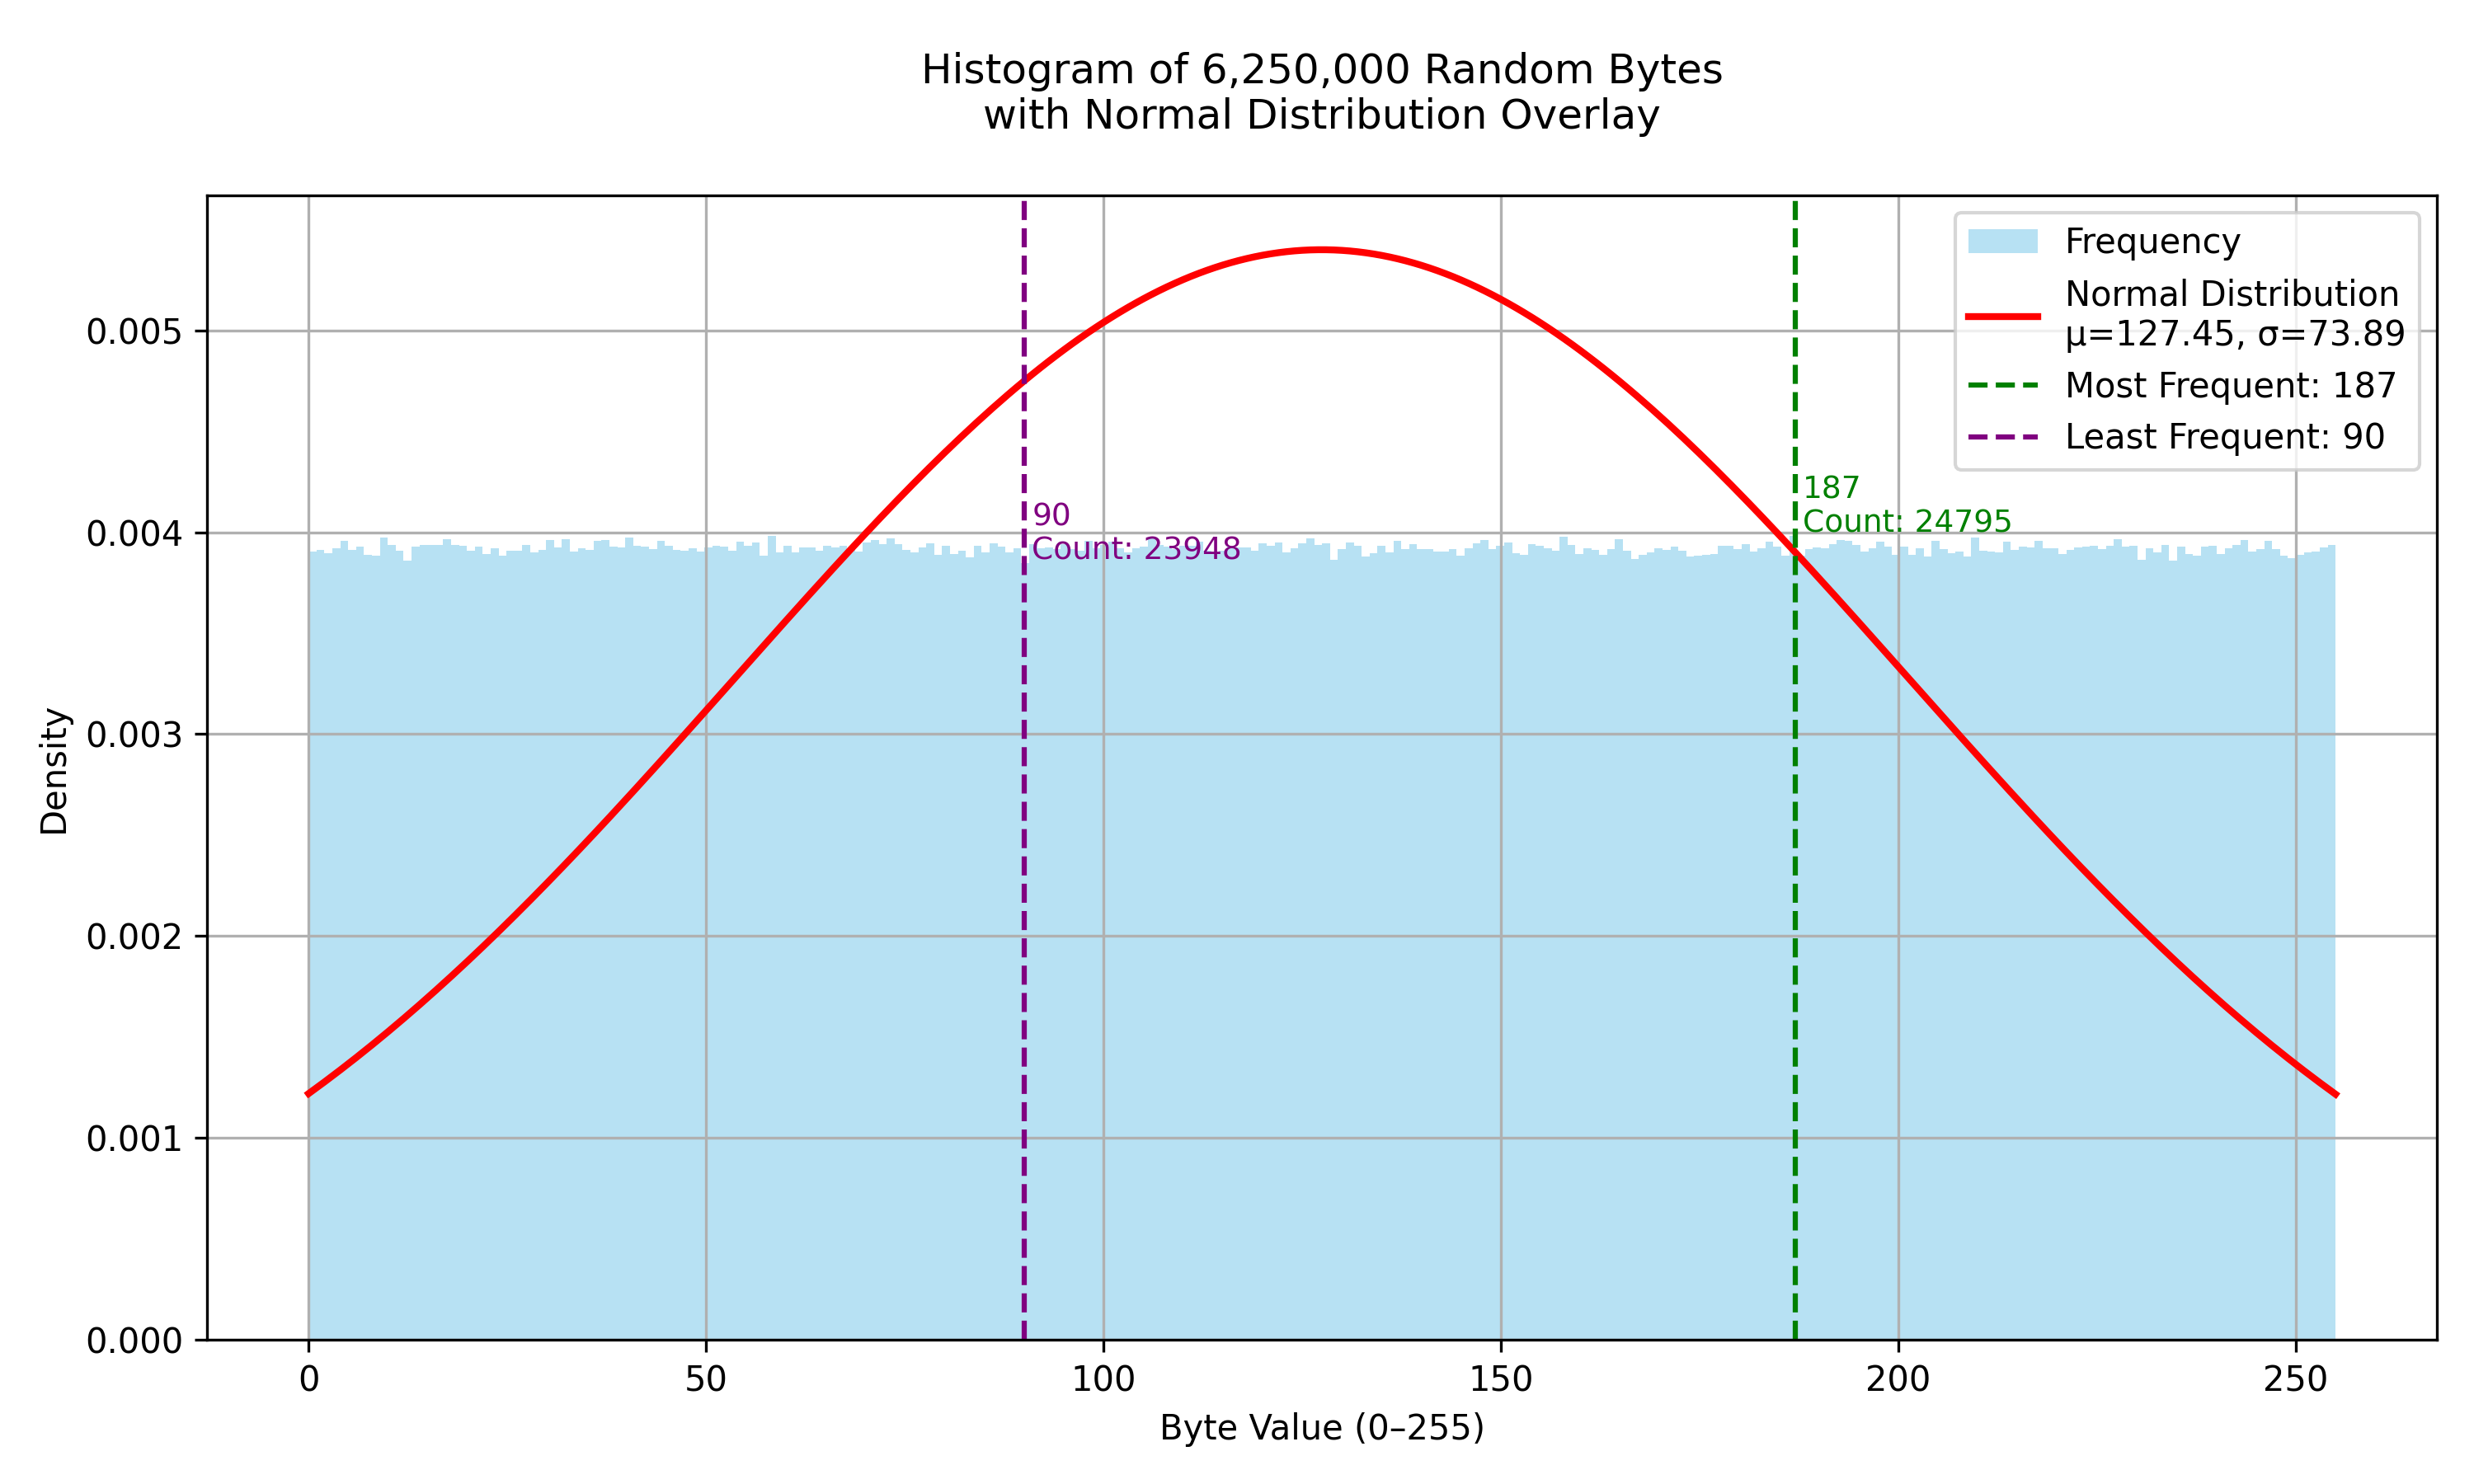
\includegraphics[width=0.9\linewidth]{images/random_bits_CTR_DRBG_seed_python_random.png}
    \caption{\raggedright Random bits \textit{CTR\_DRBG} seed generation with Python random function.}
    \label{fig:ctr_drbg_python_random}
\end{figure}


\subsection{Distribution of Random Bits Generated with Sequential Seeds}
\label{sec:distribution_sequential_seed}

For the following test, sequential seeds were used starting at 1 and reaching 6.5 million in the set of natural numbers. This number was converted to binary and turned into a 32-bit number, then it was used as a seed to generate the distribution with the \textit{CTR\_DRBG} method, showing a uniform distribution without much variation. Unexpectedly, it is seen that the distribution behaves very similar to obtaining reliable seeds with true entropy. Below is the graph.

\begin{figure}[htbp]
    \centering
    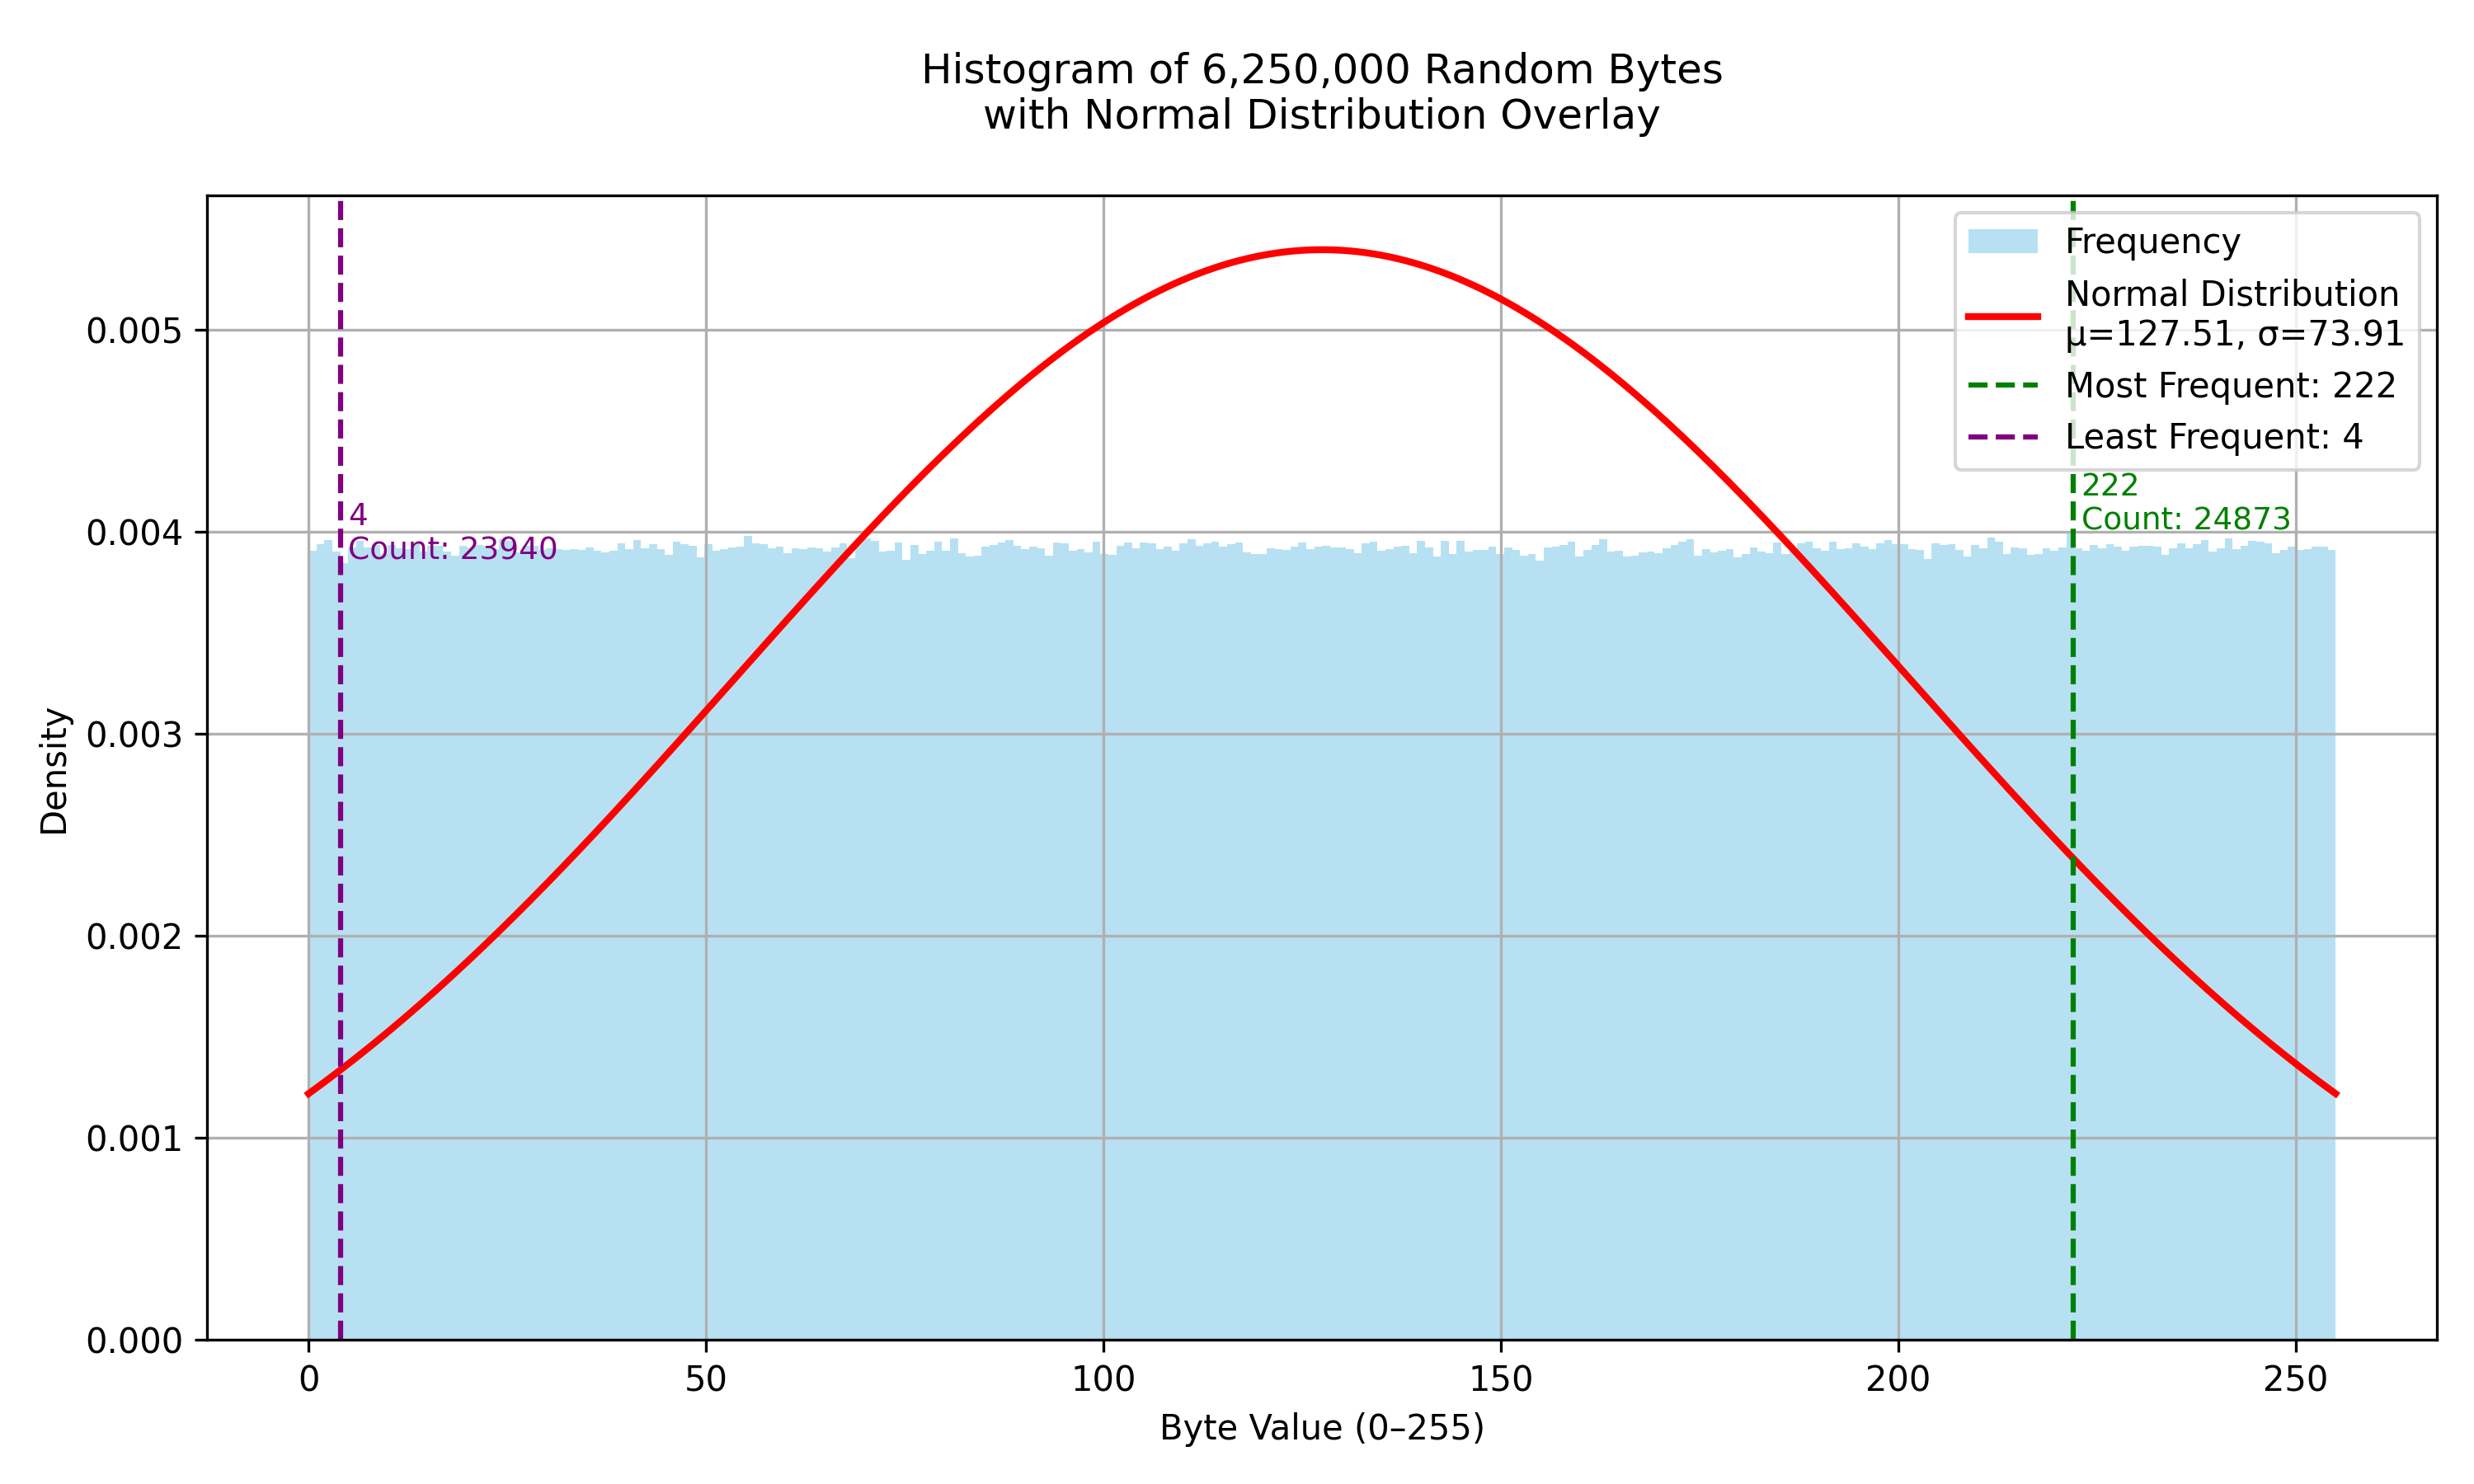
\includegraphics[width=0.9\linewidth]{images/secuentialSeedFrom0_To_100M_CTR_DRBG.png}
    \caption{\raggedright Sequential seed from 1 to 6.5M using \textit{CTR\_DRBG}.}
    \label{fig:ctr_drbg_sequential_seed}
\end{figure}


\section{Conclusions}
The comparative analysis of various random number generators, including classical pseudo-random (CRNG), Counter Mode Deterministic Random Bit Generators (CTR DRBG and CTR DRBG with sequential seeding), and a Quantum Random Number Generator (QRNG), was conducted using a selection of five statistical tests from the NIST SP 800-22 Rev 1a suite. These tests, namely the Frequency (Monobit) Test, Frequency Test within a Block, Runs Test, Maurer's "Universal Statistical" Test, and the Cumulative Sums (Cusum) Test, proved invaluable in assessing different aspects of randomness, from basic bit balance to compressibility and trend analysis . The results indicated that both CTR DRBG implementations exhibited excellent statistical properties, passing all applied tests and demonstrating characteristics consistent with high-quality random data suitable for cryptographic applications. In contrast, the evaluated QRNG, despite its theoretical underpinnings for true randomness, showed significant deviations, failing critical tests such as the Monobit, Runs, and Cusum tests, suggesting underlying biases or issues in the generation or collection process that compromise its statistical randomness for the tested 500,000-bit sequence. The classical RNG served as a baseline and generally performed well.


\bibliographystyle{plainnat}
\bibliography{references}

\end{document}
